\section{Intro}
\label{SymmetricalIntro}

Symmetrical cryptography relies on Claude Shannon's 'theory of Information':
quantify amount of information inside a theoretical channel.
\begin{center}		
	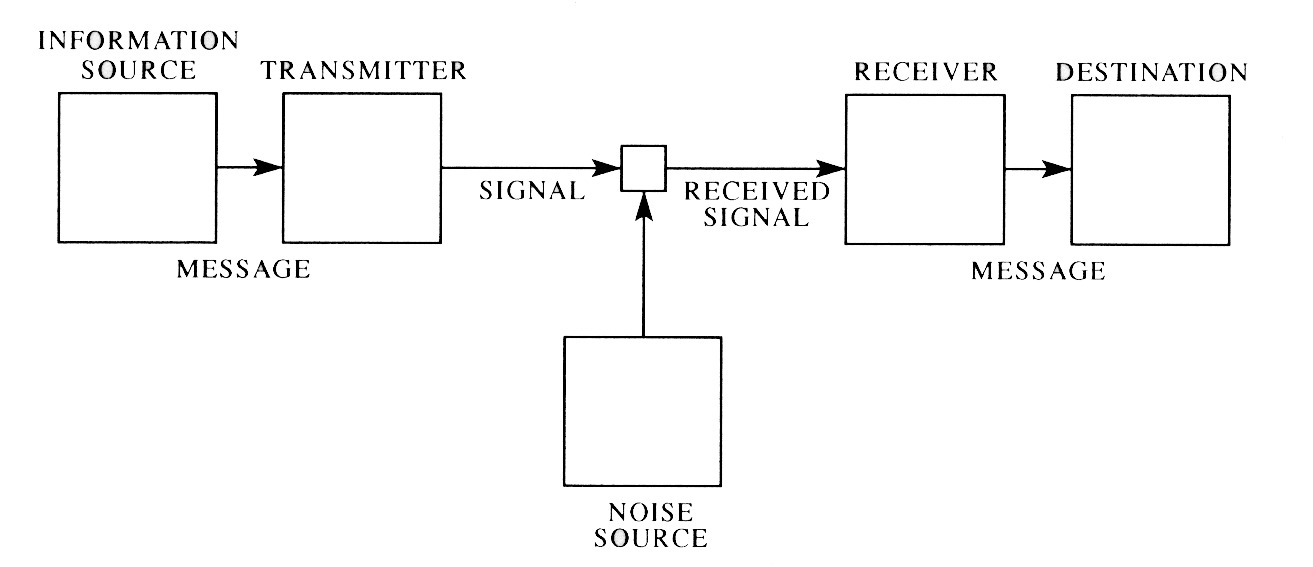
\includegraphics[width=18cm,height=5cm]{images/shannon.jpg}
\end{center}
Classical concepts: entropy, noisy channel, channel capacity, coding theory, compression. See:
\begin{itemize}
	\item Original paper  \lokiquote{sigmobile-2011-shannon}
	\item The wiki page, \href{https://en.wikipedia.org/wiki/Information_theory}{Link}
\end{itemize}
\begin{mythm}[Claude Shannon, 1948]
For any given degree of noise contamination of a communication channel, it is possible to communicate discrete data (digital information) nearly error-free up to a computable maximum rate through the channel.
\end{mythm}